\documentclass[conference]{IEEEtran}
\IEEEoverridecommandlockouts
% The preceding line is only needed to identify funding in the first footnote. If that is unneeded, please comment it out.
\usepackage[utf8]{inputenc} % allow utf-8 input
\usepackage[T1]{fontenc}    % use 8-bit T1 fonts
\usepackage{hyperref}       % hyperlinks
\usepackage{url}            % simple URL typesetting
\usepackage{booktabs}       % professional-quality tables
\usepackage{nicefrac}       % compact symbols for 1/2, etc.
\usepackage{microtype}      % microtypography
\usepackage{multicol}
\usepackage{multirow}
\usepackage{diagbox}
\usepackage{subfigure}
\usepackage{tabularx}
\usepackage{cite}
\usepackage{amsmath,amssymb,amsfonts}
\usepackage{algorithmic}
\usepackage{graphicx}
\usepackage{textcomp}
\usepackage{xcolor}
\usepackage{indentfirst}
\def\BibTeX{{\rm B\kern-.05em{\sc i\kern-.025em b}\kern-.08em
    T\kern-.1667em\lower.7ex\hbox{E}\kern-.125emX}}
\begin{document}
\bibliographystyle{IEEEtran}

\title{Principles of Data Science Project 2\\
Distance Metrics}

\author{\IEEEauthorblockN{Hongzhou Liu}
\IEEEauthorblockA{517030910214}
\texttt{deanlhz@sjtu.edu.cn}
\and
\IEEEauthorblockN{Xuanrui Hong}
\IEEEauthorblockA{517030910227}
\texttt{hongxuanrui.1999@sjtu.edu.cn}
\and
\IEEEauthorblockN{Qilin Chen}
\IEEEauthorblockA{517030910155}
\texttt{1017856853@sjtu.edu.cn}
}

\maketitle

\begin{abstract}
Hello
\end{abstract}

\begin{IEEEkeywords}
kNN, Distance Metric, Metric Learning
\end{IEEEkeywords}

\section{Introduction}
\subsection{k-Nearest Neighbor}
K-Nearest Neighbor is a kind of supervised learning method. It can be used for both classification and regression.
In the case of classification, the input consists of the $k$ closest training examples in the feature space and the output is a class membership.
A certain object is classified by a plurality vote of its neighbors, with it being assigned to the class which is the most common in its $k$ nearsest neighbors.
The algorithm is non-parametric\cite{knn}, which means the model is distribution free or with a specified distribution whose parameters are unspecified.
It is also a type of instance-based learning or lazy learning, where the generalization of the training data is delayed until a query is made. In this case, $k$-NN has no explicit 
training step and does all computations during testing period. Because we are finding the $k$ nearest neighbors, the distance metric to evaluate "nearest" is significant in $k$-NN.
\subsection{Distance Metrics}
\subsubsection{Minkowski Distance}
Minkowski Distance is a metric in normed vector space. It is a generalization of the well-known Euclidean distance, the Manhattan distance and the Chebyshev distance.
The Minkowski distance of order $p$ between two points $\mathbf{x}=(x_1,x_2,\cdots,x_n), \mathbf{y}=(y_1,y_2,\cdots,y_n) \in \mathbb{R}^n$ is defined as
\begin{equation}
    d(\mathbf{x}, \mathbf{y})=\left(\sum_{i=1}^{n}\left|x_{i}-y_{i}\right|^{p}\right)^{\frac{1}{p}}
\end{equation}
The following figure \ref{fig:mkd} shows unit circles (the set of all points which are at the unit distance from the center) with different values of $p$.
\begin{figure}[htbp]
	\centering
	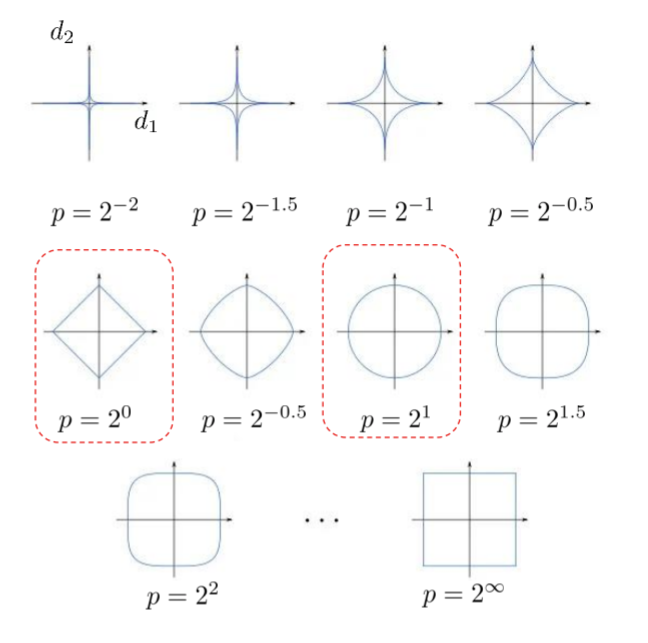
\includegraphics[scale=0.3]{pic/minkowski.png}
	\caption{Unit Circles}
	\label{fig:mkd}
\end{figure}
\subsubsection{Chebyshev Distance}
The Chebyshev distance or $L_{\infty}$ metric is a metric defined on a vector space where the distance between two points is the maximum of their differences along any coordinate dimension.\cite{hmds}
It is actually the Minkowski distance when $p\rightarrow\infty$ and thus is defined as:
\begin{equation}
    d_{Chebyshev}(\mathbf{x},\mathbf{y})=\lim_{p\rightarrow\infty}\left(\sum_{i=1}^{n}\left|x_{i}-y_{i}\right|^{p}\right)^{\frac{1}{p}}=\max_{i}(|x_i-y_i|)
\end{equation}
\subsubsection{Euclidean Distance}
The Euclidean distance is the "ordinary" straight-line distance in Euclidean space. It is also a specialization of Minkowski distance where $p=2$. Thus, it is defined as
\begin{equation}
    d_{Euclidean}(\mathbf{x},\mathbf{y})=\sqrt{\sum_{i=1}^n(x_i-y_i)^2}
\end{equation}
\subsubsection{Manhattan Distance}
The Manhattan distance is a metric in which the distance between two points is the sum of the abosolute differences of their Cartesian coordinates. The name alludes to the island of Manhattan, which causes the shortest paths a
car could take between two intersections to have the same length \ref{fig:mah}. As it's the Minkowski distance with $p=1$, it is defined as:
\begin{equation}
    d_{Manhattan}(\mathbf{x},\mathbf{y})=\left|\sum_{i=1}^n(x_i-y_i)\right|
\end{equation}
\begin{figure}[htbp]
	\centering
	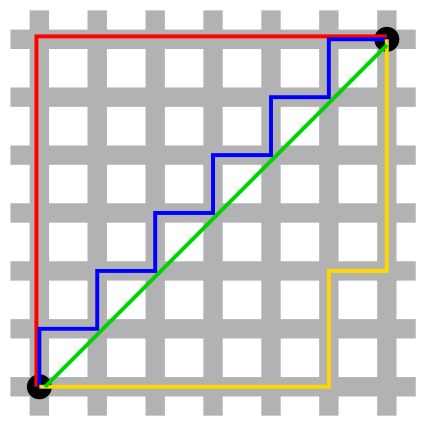
\includegraphics[scale=0.3]{pic/manhattan.png}
	\caption{Manhattan vs Euclidean}
	\label{fig:mah}
\end{figure}
\subsubsection{Cosine Distance}
The Cosine distance is closely related to Cosine similarity where the more similar two points are, the closer their distance is. The Cosine similarity between two non-zero points of an inner product space is defined to equal to the cosine of
the angle between them. Then, we can define it as:
\begin{equation}
    similarity(\mathbf{x},\mathbf{y})=\dfrac{\langle\mathbf{x},\mathbf{y}\rangle}{\|\mathbf{x}\| \|\mathbf{y}\|}=\dfrac{\sum_{i=1}^n x_i y_i}{\sqrt{\sum_{i=1}^n x_i^2}\sqrt{\sum_{i=1}^n y_i^2}}
\end{equation}
Thus, the Cosine distance is defined as:
\begin{equation}
    d_{cosine}(\mathbf{x},\mathbf{y})=1-similarity(\mathbf{x},\mathbf{y})
\end{equation}
\subsubsection{Mahalanobis Distance}
\subsection{Metric Learning}
\section{Simple Distance Metrics}
\section{Metric Learning}
\subsection{Information Theoretic Metric Learning (ITML)}
% ITML is an information-besed learning approach taht formulate the problem as that of minimizing the differential relative entropy between two multivariate Gaussians under constraints on the distance function\cite{Davis2007Information}. In this section, we will introduce the experiment on pure ITML, PCA-preprocessed ITML and LDA-preprocessed ITML.

In this experiment, we trained supervised ITML model in training dataset, then transform source data to ITML-learned data for KNN classification. We set $constraints=200$ in supervised ITML model and give the $k-$neighbors range in $k-$NN model as $[2, 3, 4, 5, 6, 7, 8, 9, 10, 11, 12, 13, 14, 15, 16]$. For PCA-preprocessed ITML, we first perprocess the data by 50-conponents linear PCA, then train supervised ITML model on the processed data, it will give a better performance. For LDA-preprocessed one, we perprocess the data by 40-conponents LDA, instead.

\begin{table}[htbp]
	\centering
 	\newcommand{\tabincell}[2]{\begin{tabular}{@{}#1@{}}#2\end{tabular}}
 	\renewcommand\arraystretch{1.0}
 	\caption{Comparison of Variance ITML and baselines in $k-$NN Classification Task}
 	\label{base2}%
 		\begin{tabular}{@{}p{1cm}<{\centering}|c|c|c}
 		\hline
 		\multirow{2}{*}{\diagbox[height=2\line,width=1.42cm,font=\tiny]{$k$}{Acc.}{$\mathit{M}$}} &
 		\multicolumn{3}{c}{Variance ITML model + $k-$NN}\\
 		\cline{2-4}
 		& {ITML(\%)} & {PCA-preprocessed(\%)} & {LDA-preprocessed(\%)}\\
 		\hline
 		2   & 82.04 & 83.18 & 88.06\\
 		\hline
 		3   & \textbf{83.60} & 85.41 & 89.57\\
 		\hline
 		4   & 83.31 & 85.55 & 89.42\\
 		\hline
 		5   & 83.52  & 86.19 & 90.01\\
 		\hline
 		6   & 83.33  & 86.21 & 90.04\\
 		\hline
 		7   & 83.37  & \textbf{86.67} & 90.35\\
 		\hline
 		8   & 83.02  & 86.51 & 90.35\\
 		\hline
 		9   & 82.97  & 86.37 & 90.40\\
 		\hline
 		10   & 82.72  & 86.41 & 90.55\\
 		\hline
 		11   & 82.73  & 86.25 & 90.64\\
 		\hline
 		12   & 82.52  & 86.27 & 90.67\\
 		\hline
 		13   & 82.47  & 86.17 & 90.58\\
 		\hline
 		14   & 82.33  & 86.06 & 90.64\\
 		\hline
 		15   & 82.10  & 86.15 & \textbf{90.74}\\
 		\hline
 		16   & 81.96  & 86.01 & 90.69\\
 		% \hline Baseline& \multicolumn{3}{c}{87.61} \\
 		\hline
 	\end{tabular}
\end{table}

Our experiment results are shown in Tab. \ref{base2}. Compared with baseline $87.61\%$ in Euclidean KNN, we can find that simple ITML model and PCA-preprocessed ITML model have poor performance, we deem the reason is that ITML minimize the LogDet divergence subject to linear constraints while it does not rely on an eigenvalue computation, and PCA can't differ the classes which is useless for $k-$NN classification. But we can find PCA-preprocessed model have better performance than pure ITML model, we think PCA method can have compensation on eigenvalue computation for ITML. When we set $k=15$, we have best performance $90.74\%$, we think LDA method can make the variance high enough between different clusters. 


\subsection{Local Fisher Discriminant Analysis (LFDA)}

% Local Fisher Discriminant Analysis (LFDA) \cite{Sugiyama2008Semi} is a linear supervised dimensionality reduction method while ITML tends to be information-based method. LFDA extends LDA by assigning greater weights to those connecting examples that are nearby rather than distant. It is particularly useful when dealing with multimodality, where one ore more classes consist of separate clusters in input space. In this section, we will introduce the experiment on pure LFDA, PCA-preprocessed LFDA and LDA-preprocessed LFDA.

In this experiment, we trained LFDA model in training dataset, then project source data to LFDA-learned data for KNN classification. We set $k-$neighbors range in $k-$NN model as $[2, 3, 4, 5, 6, 7, 8, 9, 10, 11, 12, 13, 14, 15, 16]$. For PCA-preprocessed LFDA, we first perprocess the data by 50-conponents linear PCA, then train supervised ITML model on the processed data, it will give a better performance. For LDA-preprocessed one, we perprocess the data by 40-conponents LDA, instead.

\begin{table}[htbp]
	\centering
 	\newcommand{\tabincell}[2]{\begin{tabular}{@{}#1@{}}#2\end{tabular}}
 	\renewcommand\arraystretch{1.0}
 	\caption{Comparison of Variance LFDA and baselines in $k-$NN Classification Task}
 	\label{base3}%
 		\begin{tabular}{@{}p{1cm}<{\centering}|c|c}
 		\hline
 		\multirow{2}{*}{\diagbox[height=2\line,width=1.42cm,font=\tiny]{$k$}{Acc.}{$\mathit{M}$}} &
 		\multicolumn{2}{c}{Variance LFDA model + $k-$NN}\\
 		\cline{2-3}
 		& {PCA-preprocessed(\%)} & {LDA-preprocessed(\%)}\\
 		\hline
 		2   & 84.00 & 88.18\\
 		\hline
 		3   & 86.30 & 89.95\\
 		\hline
 		4   & 86.74 & 89.94\\
 		\hline
 		5   & 87.17 & 90.38\\
 		\hline
 		6   & 87.16 & 90.29\\
 		\hline
 		7   & 87.40 & 90.43\\
 		\hline
 		8   & 87.42 & 90.54\\
 		\hline
 		9   & 87.51 & 90.62\\
 		\hline
 		10   & 87.46 & 90.55\\
 		\hline
 		11   & \textbf{87.51} & 90.63\\
 		\hline
 		12   & 87.38 & 90.68\\
 		\hline
 		13   & 87.49 & 90.71\\
 		\hline
 		14   & 87.24 & 90.68\\
 		\hline
 		15   & 87.23 & \textbf{90.76}\\
 		\hline
 		16   & 86.97 & 90.76\\
 		% \hline Baseline& \multicolumn{3}{c}{87.61} \\
 		\hline
 	\end{tabular}
\end{table}

Our experiment results are shown in Tab. \ref{base3}. We find simple LFDA model have poor performance as $16.20\%$, we think this may be caused by that we set the n\_components parameter as default, and it means we can't control its dimensionality reduction process to get a satisfied result. Compared with baseline $87.61\%$ in Euclidean KNN, we find LDA-preprocessed model reached $90.76\%$ while PCA-preprocessed one reached $87.51\%$, we deem the reason is that LDA can make the variance high enough between different clusters.

\section{Conclusion}

In this project, we introduced traditional distance metric and several metric learning method, which is to learn a distance metric for the input space of data from a given collection of pair of similar/dissimilar points that preserves the distance relation among the training data. We have several supervised experiments such as ITML, LFDA, MMC, RCA and LMNN, and give a experiment with unsupervised method PCA. In this section, we will conclude the properties of every method and conclude the performance of simple distance metrics and metrics learning models.

PCA is a supervised dimensionality reduction method, which can preserve the global structure and maintain the variance of the data. In our project, we use PCA to processed data, i.e. we project the data into processed data, then we can use different distance metrics in $k-$NN, such as Euclidean, Manhattan, Chebyshev and Cosine. Most importantly, we can use it to preprocess data before we use anothor metircs learning method, we use this combination method in other experiments, for example, PCA-preprocessed ITML, it means we use PCA to proprecess the data, and then use ITML to finish metrics learning before $k-$NN steps.

ITML is an information-besed learning approach that formulate the problem as that of minimizing the differential relative entropy between two multivariate Gaussians under constraints on the distance function\cite{Davis2007Information}. It does not rely on an eigenvalue computation but probability distributions, it results its performance can increase when we combine it with PCA-processed or LDA-processed.

LFDA is a linear supervised dimensionality reduction method while ITML tends to be information-based method. It extend LDA by assigning greater weights to closer connecting examples and can only maintain the local data structure. In our experiment, we combine LFDA with PCA-processed or LDA-processed method to get a satisfied result.

MMC minimizes the sum of squared distances between similar points, while enforcing the sum of distances between dissimilar ones to be greater than one. This leads to a convex and, thus, local-minima-free optimization problem that can be solved efficiently. In our experiment, we set 200 constrains for MMC evaluation, and find its satisfied performance.

RCA learns a global linear transformation from the equivalence constraints, and the learned linear transformation can be used directly to compute distance between any two examples. It can preserve global structure and all the positive/negative constrains, it means it will cost very large memory and take too long, therefore in our experiment we use PCA and LDA to preprocess the source data instead of evaluating pure RCA model.

LMNN is a linear model that extends NCA through a maximum margin framework. It learns a Mahalanobis distance that tries to collapse examples in the same class to a single point, and in the meantime keep examples from different classes far away. LMNN preserve the local information as NCA but have better performance than NCA. In our experiments, to prevent memory explosion, we only evaluate performance of LMNN model at $k-$neighbors range of $[2,3,4,5,6]$ and use PCA or LDA to preprocess the data.

\begin{center}
\begin{figure}
\centering
\subfigure[PCA 2D-scattering]{
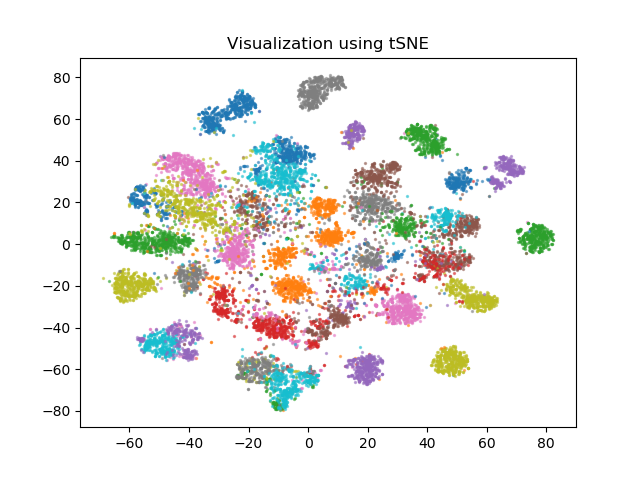
\includegraphics[width=3.75cm]{pic/X_test_scatter_PCA.png}
%\caption{fig1}
}
\quad
\subfigure[LDA 2D-scattering]{
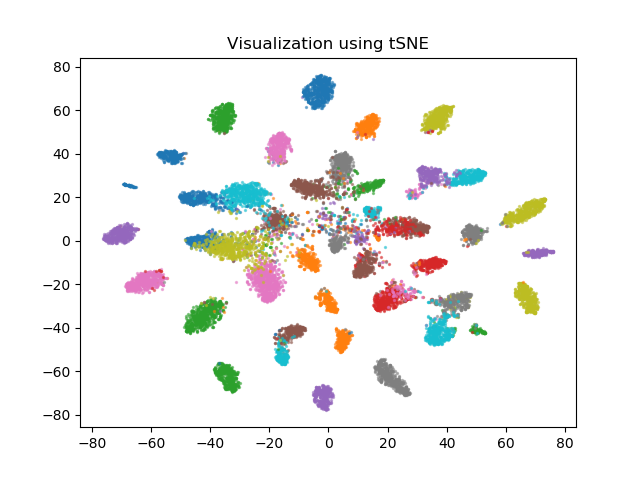
\includegraphics[width=3.75cm]{pic/X_test_scatter_LDA.png}
}
\quad
\subfigure[PCA + MMC 2D-scattering]{
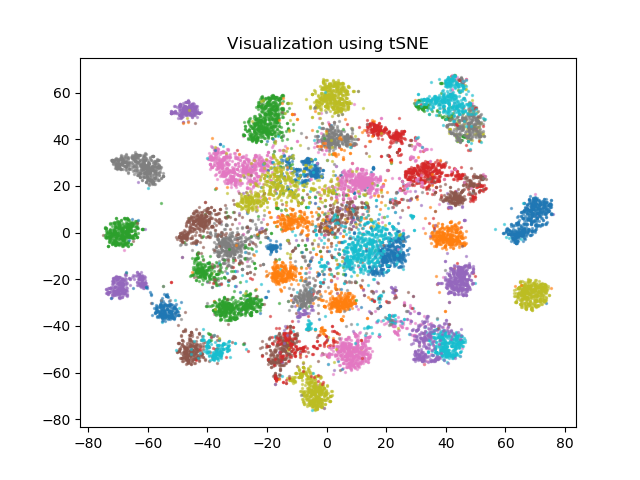
\includegraphics[width=3.75cm]{pic/X_test_scatter_PCA_MMC.png}
}
\quad
\subfigure[LDA + MMC 2D-scattering]{
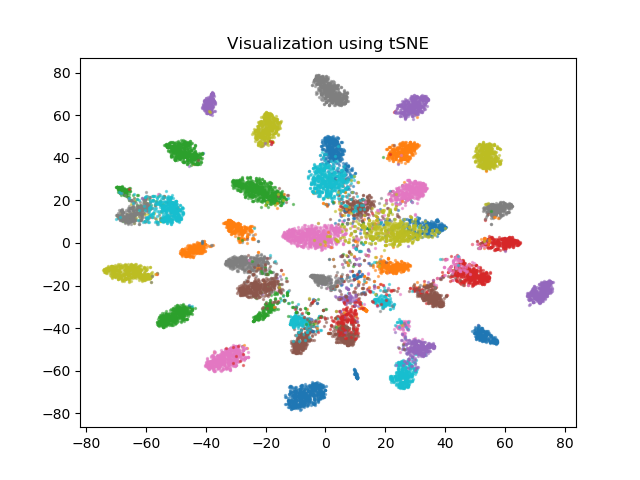
\includegraphics[width=3.75cm]{pic/X_test_scatter_LDA_MMC.png}
}
\caption{tSNE Visualization with Variance Model}
\label{Fig2}
\end{figure}
\end{center}

\bibliography{Prj2}
\end{document}
